% Clean pipeline schematic (replaces the messy Matplotlib figure).
% Compile:  pdflatex pipeline_figure.tex  ->  pipeline_figure.pdf
% Then copy pipeline_figure.pdf over pipeline.pdf.
\documentclass[border=8pt]{standalone}
\usepackage[T1]{fontenc}
\usepackage{amsmath}
\usepackage{tikz}
\usetikzlibrary{arrows.meta,positioning,fit,backgrounds}

\begin{document}
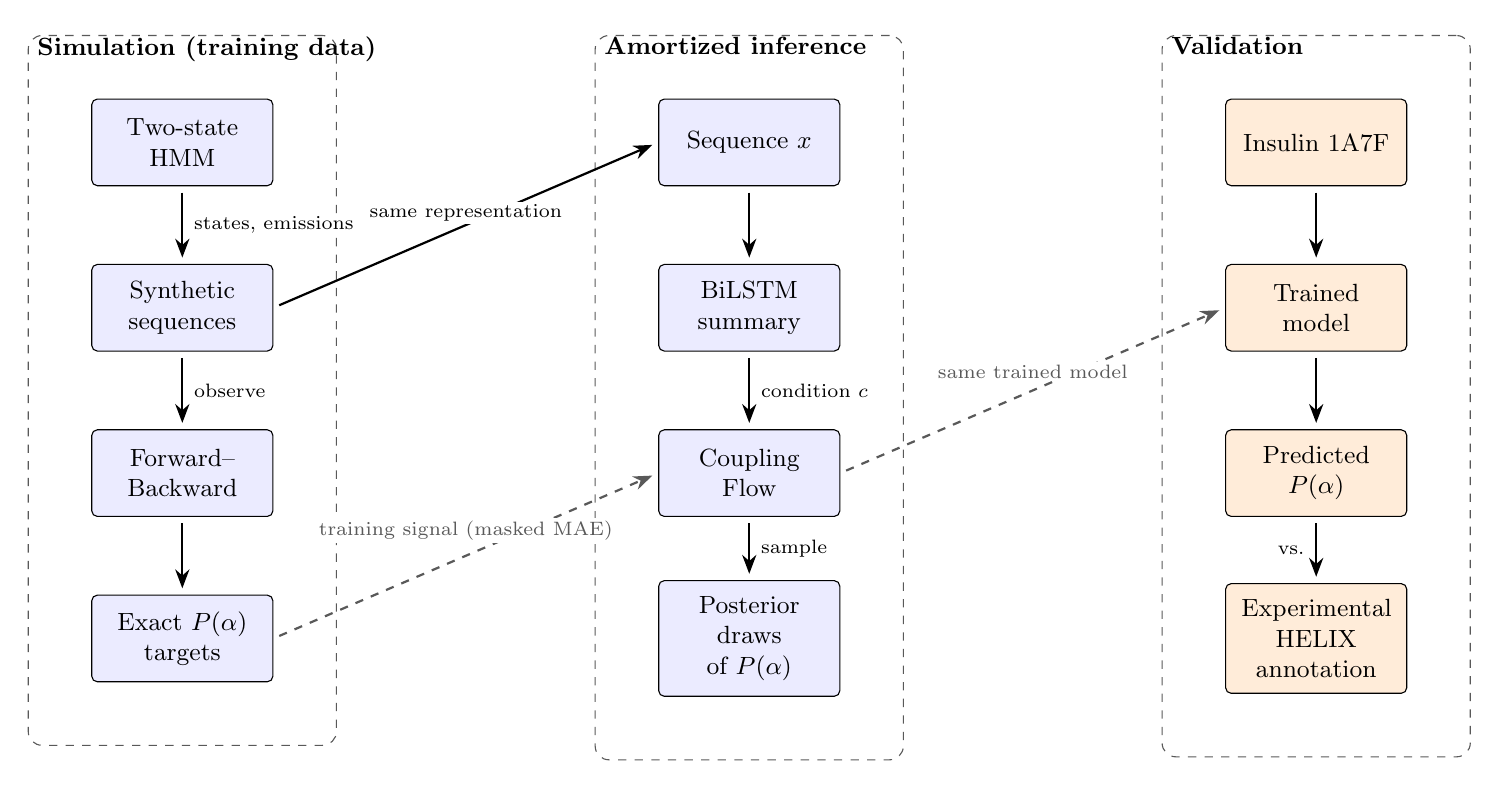
\begin{tikzpicture}[
  font=\small,
  node distance=0mm,
  blk/.style={draw, rounded corners=2pt, fill=blue!8,
              text width=19mm, minimum height=11mm, align=center, inner sep=2mm},
  org/.style={draw, rounded corners=2pt, fill=orange!15,
              text width=19mm, minimum height=11mm, align=center, inner sep=2mm},
  stg/.style={draw=black!65, rounded corners=5pt, dashed, inner sep=8mm},
  arr/.style={-{Stealth[length=2.4mm]}, thick, shorten >=0.8mm, shorten <=0.8mm},
  darr/.style={arr, dashed, black!65},
  lbl/.style={font=\scriptsize, fill=white, inner sep=1pt},
]

% ---------------- Simulation column (left) ----------------
\node[blk] (hmm)   at (3.4, 6.3) {Two-state HMM};
\node[blk] (seq)   at (3.4, 4.2) {Synthetic sequences};
\node[blk] (fb)    at (3.4, 2.1) {Forward--Backward};
\node[blk] (exact) at (3.4, 0.0) {Exact $P(\alpha)$ targets};

\draw[arr] (hmm.south) -- (seq.north) node[lbl, midway, right=1mm] {states, emissions};
\draw[arr] (seq.south) -- (fb.north)  node[lbl, midway, right=1mm] {observe};
\draw[arr] (fb.south)  -- (exact.north);

% ---------------- Amortized inference column (middle) ----------------
\node[blk] (x)    at (10.6, 6.3) {Sequence $x$};
\node[blk] (sum)  at (10.6, 4.2) {BiLSTM summary};
\node[blk] (flow) at (10.6, 2.1) {Coupling Flow};
\node[blk] (post) at (10.6, 0.0) {Posterior draws of $P(\alpha)$};

\draw[arr] (x.south)    -- (sum.north);
\draw[arr] (sum.south)  -- (flow.north) node[lbl, midway, right=1mm] {condition $c$};
\draw[arr] (flow.south) -- (post.north) node[lbl, midway, right=1mm] {sample};

% ---------------- Validation column (right) ----------------
\node[org] (ins)   at (17.8, 6.3) {Insulin 1A7F};
\node[org] (model) at (17.8, 4.2) {Trained model};
\node[org] (pred)  at (17.8, 2.1) {Predicted $P(\alpha)$};
\node[org] (helix) at (17.8, 0.0) {Experimental HELIX annotation};

\draw[arr] (ins.south)   -- (model.north);
\draw[arr] (model.south) -- (pred.north);
\draw[arr] (pred.south)  -- (helix.north) node[lbl, midway, left=1mm] {vs.};

% ---------------- Cross-stage links ----------------
\draw[arr]  (seq.east)   -- (x.west)   node[lbl, midway, above] {same representation};
\draw[darr] (exact.east) -- (flow.west) node[lbl, midway, above=1.5mm] {training signal (masked MAE)};
\draw[darr] (flow.east)  -- (model.west) node[lbl, midway, above=1mm] {same trained model};

% ---------------- Stage frames ----------------
\begin{scope}[on background layer]
  \node[stg, fit=(hmm)(seq)(fb)(exact)] (s1) {};
  \node[stg, fit=(x)(sum)(flow)(post)]   (s2) {};
  \node[stg, fit=(ins)(model)(pred)(helix)] (s3) {};
  \node[anchor=north west, font=\small\bfseries, yshift=1mm] at (s1.north west) {Simulation (training data)};
  \node[anchor=north west, font=\small\bfseries, yshift=1mm] at (s2.north west) {Amortized inference};
  \node[anchor=north west, font=\small\bfseries, yshift=1mm] at (s3.north west) {Validation};
\end{scope}

\end{tikzpicture}
\end{document}
